Consider the positive-feedback circuit shown in Figure: \ref{fig:ee18btech11030}. 
\begin{enumerate}
\item Find the loop transmission L(s) and the characteristic equation
\item Find the expressions for resulting pole frequency $\omega_o$ and Q factor?
\item Sketch a Pole-Zero plot for varying K. For what value of K do the poles coincide? For what value of K does the response becomes maximally flat? For what value of K does the circuit oscillate?
\end{enumerate}
 Assume that the amplifier has frequency-independent gain, infinite input impedance, and zero output impedance.
\begin{figure}[!ht]
	\begin{center}
		\resizebox{\columnwidth/1}{!}{ 
\usetikzlibrary{decorations.markings}
\begin{circuitikz}
\draw (-4,-1) to[amp,t={+K}] (2.5,-1);
\draw (-4,-1) to (-4,2) to (-3,2) ;
\draw (-3,2)  to [capacitor=$C/10$](-3,0.5) to  (-3,0.5) node[ground]{};
\draw (-3,2) to (-2.3,2)to [R=$10R$] (-1.3,2)to (0,2) to [R=$R$] (0,5) node[label={}]{}  to (-4,5) ;
\draw (0,2) to(1,2) to  [capacitor=$C$](1.5,2) to (2.5,2) to (2.5,-1);
\draw (-4,5) to (-4,4.7) to [V=$V_s$] (-4,3.9) to (-4,3.5) node[ground]{} ;
\draw (2.5,-1) to[short, -o] (3,-1) node[label={above:$V_{out}$}]{};
\end{circuitikz}}
	\end{center}
	\caption{ Positive Feedback Circuit}
	\label{fig:ee18btech11030}
\end{figure}
\begin{enumerate}[label=\arabic*.,ref=\theenumi]
%\begin{enumerate}[label=\thesubsection.\arabic*.,ref=\thesubsection.\theenumi]
\numberwithin{equation}{enumi}
\item 

\solution To obtain the loop transmission L(s),
\begin{itemize}
\item Short-circuit the signal source $V_s$.
\item Break the loop at the Amplifier input.
\item Then apply a test voltage $V_t$ and find the returned voltage $V_r$, as indicated in Figure: \ref{fig:ee18btech11030_fig1}.
\end{itemize}

\begin{figure}[!ht]
	\begin{center}
		\resizebox{\columnwidth/1}{!}{\usetikzlibrary{decorations.markings}
\begin{circuitikz}
\draw (-2,0) to[amp,t={+K}] (3,0);
\draw (3,0) to (3,4) to [capacitor=$C$](1.7,4) to (1,4)  to [R=$R$] (1,2) to (1,2) node[ground]{} ;
\draw (3,4) to [short, -o] (3.5,4) node[label={above:$V_{1}$}]{} ;
\draw [dashed] (2.8,1) to (-1.5,1) to (-1.5,4.5) to (2.8,4.5) to (2.8,1); 
\draw (1,4) to  [R=$10R$] (-1,4) to [capacitor=$C/10$](-1,2) to (-1,2) node[ground]{} ;
\draw (-1,4) to [short, -o] (-2,4) node[label={above:$V_{r}$}]{};
\draw (-2,0) to [short, -o] (-3,0) node[label={above:$V_{t}$}]{} ;
\end{circuitikz}
}
	\end{center}
	\caption{}
	\label{fig:ee18btech11030_fig1}
\end{figure}

The loop transmission is given by
\begin{align}
    L\brak{s} = -\frac{V_r\brak{s}}{V_t\brak{s}} = -KT\brak{s}
\label{eq:ee18btech11030}
\end{align}
where T(s) is the transfer function of the two-port RC network shown inside the broken-line box in Figure: \ref{fig:ee18btech11030_fig1}.

\begin{align}
T\brak{s} = \frac{V_r\brak{s}}{V_1\brak{s}}
\label{eq:ee18btech11030_1}
\end{align}
Applying KCL at nodes present in the RC network yields  
\begin{align}
T\brak{s} = \frac{s(\frac{1}{CR})}{s^2 + s(\frac{2.1}{CR}) + (\frac{1}{CR})^2}
\label{eq:ee18btech11030_2}
\end{align}
Substituting T\brak{s} in Eq: \ref{eq:ee18btech11030}
\begin{align}
    L\brak{s} = \frac{-s(\frac{K}{CR})}{s^2 + s(\frac{2.1}{CR}) + (\frac{1}{CR})^2}
\end{align}
The characteristic equation is 
\begin{align}
    1+L\brak{s}=0  
\end{align}
\begin{align}
s^2 + s(\frac{2.1-K}{CR}) + (\frac{1}{CR})^2 = 0
\label{eq:ee18btech11030_3}
\end{align}
The standard characteristic equation of a second order network can be written as 
\begin{align}
    s^2 + \frac{\omega_o}{Q}s + \omega_o^2 = 0
    \label{eq:ee18btech11030_4}
\end{align}
$\omega_o$ is called pole frequency , Q is called pole Qfactor. 
By comparing the Eq:\ref{eq:ee18btech11030_3} with the standard characteristic equation Eq:\ref{eq:ee18btech11030_4}
\begin{align}
   \omega_o = \frac{1}{RC} ; Q = \frac{1}{2.1-K}
\end{align}
Closed Loop gain 
\begin{align}
    T = \frac{s(\frac{-K}{RC})}{s^2 + s(\frac{2.1-K}{CR}) + (\frac{1}{CR})^2}
    \label{eq:ee18btech11030_5}
\end{align}
\item Sketch the Normalised closed loop gain of above two pole feedback amplifier for various Q values

\solution 
\begin{figure}[!h]
\centering
  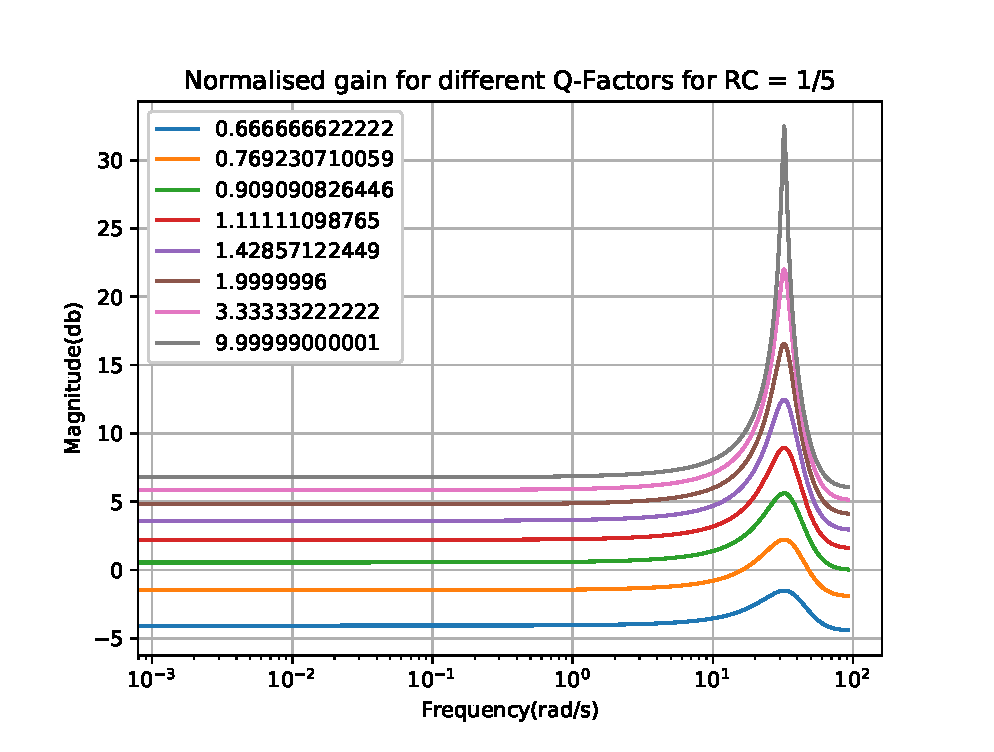
\includegraphics[width=\columnwidth]{./figs/ee18btech11030/ee18btech11030_fc.eps}
\caption{}
\label{fig:ee18btech11030_fig2} 
\end{figure}

The following is code for the plot
\begin{lstlisting}
codes/ee18btech11030/ee18btech11030.py
\end{lstlisting}
From Figure:\ref{fig:ee18btech11030_fig2} ,
\begin{itemize}
\item It is observed that maximally flat response is obtained when Q = 0.71
\item It will be seen that response of the feedback amplifier under consideration shows almost no peaking for Q$\leq$ 0.71 
\end{itemize}
\item Sketch a Pole-Zero Plot to Eq:\ref{eq:ee18btech11030_5} for a varying K

\solution :
\begin{figure}[!ht]
\centering
  \includegraphics[width=\columnwidth]{./figs/ee18btech11030/ee18btech11030_fc1.eps}
\caption{}
\label{fig:ee18btech11030_fig3} 
\end{figure}

The following is code for the  plot
\begin{lstlisting}
codes/ee18btech11030/ee18btech11030_1.py
\end{lstlisting}
From Figure : \ref{fig:ee18btech11030_fig3} 
\begin{itemize}
\item For K = 0,the poles have Q = 0.476 and therefore located on negative real axis. 
\item As K increases poles are brought closer together and eventually coincide at K = 0.1 and Q = 0.5
\item Further increase in K results in poles becoming complex conjugate 
\item Maximally flat response is obtained when Q = 0.707,which results when K = 0.686.In this case poles are at 45\degree .
\item Oscillating response is obtained when poles are completely imaginary when Q = inf which results when K = 2.1 
\end{itemize}
\item Verify the response in time domain for a unit impulse input 

\solution :
\begin{figure}[!ht]
\centering
  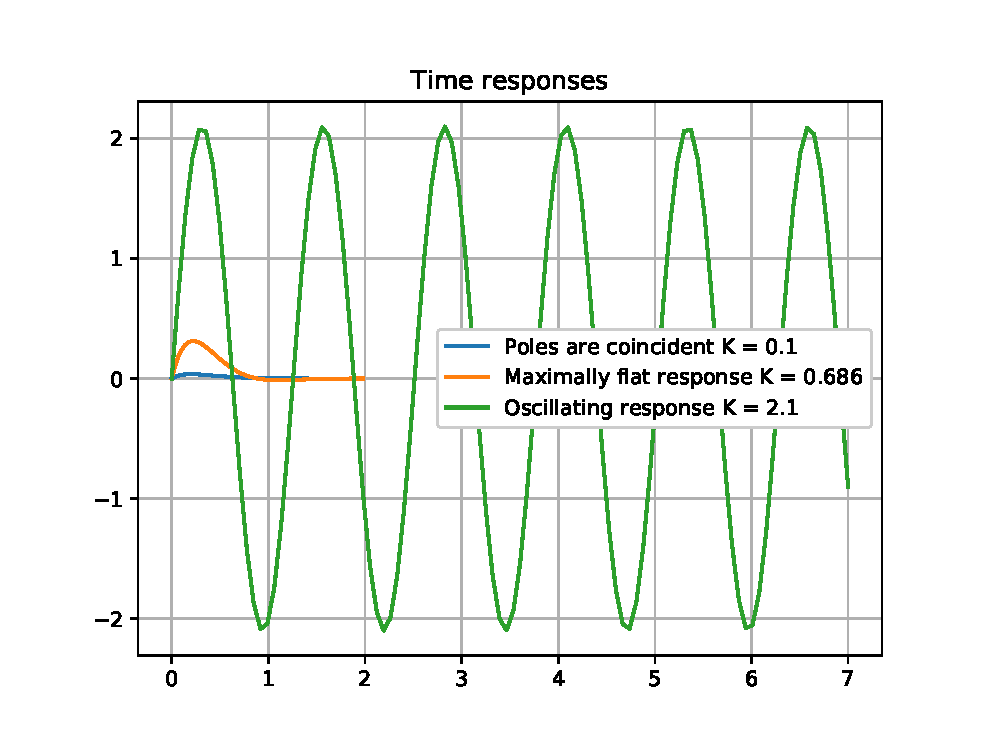
\includegraphics[width=\columnwidth]{./figs/ee18btech11030/ee18btech11030_fc2.eps}
\caption{}
\label{fig:ee18btech11030_fig4} 
\end{figure}

The following is code for the plot
\begin{lstlisting}
codes/ee18btech11030/ee18btech11030_2.py
\end{lstlisting}
\begin{table}[!ht]
\centering
 
\usetikzlibrary{decorations.markings}
\begin{circuitikz}
\draw (-4,-1) to[amp,t={+K}] (2.5,-1);
\draw (-4,-1) to (-4,2) to (-3,2) ;
\draw (-3,2)  to [capacitor=$C/10$](-3,0.5) to  (-3,0.5) node[ground]{};
\draw (-3,2) to (-2.3,2)to [R=$10R$] (-1.3,2)to (0,2) to [R=$R$] (0,5) node[label={}]{}  to (-4,5) ;
\draw (0,2) to(1,2) to  [capacitor=$C$](1.5,2) to (2.5,2) to (2.5,-1);
\draw (-4,5) to (-4,4.7) to [V=$V_s$] (-4,3.9) to (-4,3.5) node[ground]{} ;
\draw (2.5,-1) to[short, -o] (3,-1) node[label={above:$V_{out}$}]{};
\end{circuitikz}
\caption{}
\label{table:ee18btech11030_table}
\end{table}
\end{enumerate}
